\documentclass{article}
\usepackage[utf8]{inputenc}
\usepackage{graphics}
\usepackage{kvmap}
\usepackage{hyperref}
\usepackage{multicol}
\title{BCD to GRAY CONVERSION}
\author{Navya Valmeekam}
\date{August 2022}

\begin{document}

\maketitle
%\documentclass{article}
%\usepackage{setspace}
%\usepackage{gensymb}

%\singlespacing
%\usepackage[cmex10]{amsmath}

%\usepackage{amsthm}

%\usepackage{mathrsfs}
%\usepackage{txfonts}
%\usepackage{stfloats}
%\usepackage{bm}
%\usepackage{cite}
%\usepackage{cases}
%\usepackage{subfig}

%\usepackage{longtable}
%\usepackage{multirow}

%\usepackage{enumitem}
%\usepackage{mathtools}
%\usepackage{steinmetz}
%\usepackage{tikz}
%\usepackage{circuitikz}
%\usepackage{verbatim}
%\usepackage{tfrupee}
%\usepackage[breaklinks=true]{hyperref}
%\usepackage{graphicx}
%\usepackage{tkz-euclide}
%\usepackage{float}

%\usetikzlibrary{calc,math}
%\usepackage{listings}
 %   \usepackage{color}                                            %%
  %  \usepackage{array}                                            %%
   % \usepackage{longtable}                                        %%
   % \usepackage{calc}                                             %%
    %\usepackage{multirow}                                         %%
    %\usepackage{hhline}                                           %%
    %\usepackage{ifthen}                                           %%
    %\usepackage{lscape}     
%\usepackage{multicol}
%\usepackage{chngcntr}

%\DeclareMathOperator*{\Res}{Res}

\renewcommand\thesection{\arabic{section}}
\renewcommand\thesubsection{\thesection.\arabic{subsection}}
\renewcommand\thesubsubsection{\thesubsection.\arabic{subsubsection}}


\renewcommand\thesectiondis{\arabic{section}}
\renewcommand\thesubsectiondis{\thesectiondis.\arabic{subsection}}
\renewcommand\thesubsubsectiondis{\thesubsectiondis.\arabic{subsubsection}}


\hyphenation{op-tical net-works semi-conduc-tor}
\def\inputGnumericTable{}                                 %%

\lstset{
%language=C,
%frame=single, 
%breaklines=true,
%columns=fullflexible
}
%\begin{document}

\begin{multicols}{2}
\newtheorem{theorem}{Theorem}[section]
\newtheorem{problem}{Problem}
\newtheorem{proposition}{Proposition}[section]
\newtheorem{lemma}{Lemma}[section]
\newtheorem{corollary}[theorem]{Corollary}
\newtheorem{example}{Example}[section]
\newtheorem{definition}[problem]{Definition}

\newcommand{\BEQA}{\begin{eqnarray}}
\newcommand{\EEQA}{\end{eqnarray}}
\newcommand{\define}{\stackrel{\triangle}{=}}
\newcommand\hlight[1]{\tikz[overlay, remember picture,baseline=-\the\dimexpr\fontdimen22\textfont2\relax]\node[rectangle,fill=blue!50,rounded corners,fill opacity = 0.2,draw,thick,text opacity =1] {$#1$};}
\bibliographystyle{IEEEtran}
\providecommand{\mbf}{\mathbf}
\providecommand{\pr}[1]{\ensuremath{\Pr\left(#1\right)}}
\providecommand{\qfunc}[1]{\ensuremath{Q\left(#1\right)}}
\providecommand{\sbrak}[1]{\ensuremath{{}\left[#1\right]}}
\providecommand{\lsbrak}[1]{\ensuremath{{}\left[#1\right.}}
\providecommand{\rsbrak}[1]{\ensuremath{{}\left.#1\right]}}
\providecommand{\brak}[1]{\ensuremath{\left(#1\right)}}
\providecommand{\lbrak}[1]{\ensuremath{\left(#1\right.}}
\providecommand{\rbrak}[1]{\ensuremath{\left.#1\right)}}
\providecommand{\cbrak}[1]{\ensuremath{\left\{#1\right\}}}
\providecommand{\lcbrak}[1]{\ensuremath{\left\{#1\right.}}
\providecommand{\rcbrak}[1]{\ensuremath{\left.#1\right\}}}
%\theoremstyle{remark}
\newtheorem{rem}{Remark}
\newcommand{\sgn}{\mathop{\mathrm{sgn}}}
%\providecommand{\abs}[1]{\left\vert#1\right\vert}
\providecommand{\res}[1]{\Res\displaylimits_{#1}} 
\providecommand{\norm}[1]{$\left\lVert#1\right\rVert$}
%\providecommand{\norm}[1]{\lVert#1\rVert}

\providecommand{\mtx}[1]{\mathbf{#1}}
%\providecommand{\mean}[1]{E\left[ #1 \right]}
\providecommand{\fourier}{\overset{\mathcal{F}}{ \rightleftharpoons}}
%\providecommand{\hilbert}{\overset{\mathcal{H}}{ \rightleftharpoons}}
\providecommand{\system}{\overset{\mathcal{H}}{ \longleftrightarrow}}
	%\newcommand{\solution}[2]{\textbf{Solution:}{#1}}
\newcommand{\solution}{\noindent \textbf{Solution: }}
\newcommand{\cosec}{\,\text{cosec}\,}
\providecommand{\dec}[2]{\ensuremath{\overset{#1}{\underset{#2}{\gtrless}}}}
\newcommand{\myvec}[1]{\ensuremath{\begin{pmatrix}#1\end{pmatrix}}}
\newcommand{\mydet}[1]{\ensuremath{\begin{vmatrix}#1\end{vmatrix}}}
%\numberwithin{equation}{subsection}
\makeatletter
\@addtoreset{figure}{problem}
\makeatother
\let\StandardTheFigure\thefigure
\let\vec\mathbf
\renewcommand{\thefigure}{\theproblem}
\def\putbox#1#2#3{\makebox[0in][l]{\makebox[#1][l]{}\raisebox{\baselineskip}[0in][0in]{\raisebox{#2}[0in][0in]{#3}}}}
     \def\rightbox#1{\makebox[0in][r]{#1}}
     \def\centbox#1{\makebox[0in]{#1}}
     \def\topbox#1{\raisebox{-\baselineskip}[0in][0in]{#1}}
     \def\midbox#1{\raisebox{-0.5\baselineskip}[0in][0in]{#1}}
\begin{center} 
\vspace{0cm}
\title{Assignment No.1}


\author{Valmeekam Navya}
\begin{tableofcontents}
\begin{abstract}
    This manual explains BCD to GRAY code conversion by finding boolean equations.
\end{abstract}
\section{BCD to GRAY Conversion}
The BCD to GRAY code converter takes the numbers 0, 1, . . . , 9 in binary as inputs and generates the converted number as output. Make connections as shown in table 1.
Gray code – also known as Cyclic Code, Reflected Binary Code (RBC), Reflected Binary (RB) or Grey code.
\newline
\newline
\textbf{Problem : -}
Implement BCD to GRAY conversion 
\newline
\vspace{4cm}
\newline
\newline
\newline
\newline
\newline
\textbf{Connections :-}
\newline
\newline
\begin{tabular}{|c|c|c|c|c|c|c|c|c|c|}
\hline
\textbf{Arduino} & 2 & 3 & 4 & 5 & 6 & 7 & 8  \\
\hline
\textbf{Display} & {a} & {b} & {c} & {d} & {e} & {f} & {g} \\
\hline
\end{tabular}
\newline
Table 1

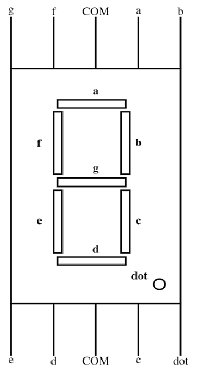
\includegraphics[scale=1]{../display.png} 
\begin{figure}[hbtp]
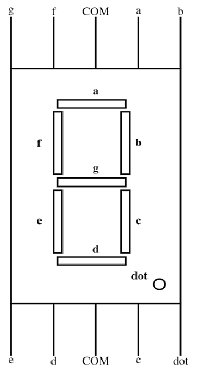
\includegraphics[scale=1]{../display.png}
%\caption{figure 1}
%\end{figure}
%\caption{figure 1}
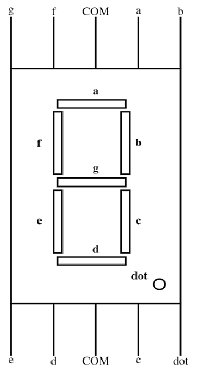
\includegraphics[scale=1]{../display.png}
\end{figure}
\begin{center}
Figure 1
\end{center}
\newpage
\section{Karnaugh Map}
Using Boolean logic or kmaps, G0, G1, G2, G3 in the truth table can be expressed in terms of the inputs A,B,C,D 
\newline
\begin{kvmap}
\begin{kvmatrix}{C,D,A,B}
0&1&0&1 \\
0&1&0&1 \\
0&0&0&0 \\
0&1&0&0 \\
\end{kvmatrix}
\bundle[color=red]{1}{0}{1}{1}
\bundle[color=red]{3}{0}{3}{1}
\bundle[color=red]{1}{3}{1}{3}
\end{kvmap}
\newline
Kmap for G0
\begin{equation}
G0=A'C'D+A'CD'+AB'C'D 
\end{equation}
\begin{kvmap}
\begin{kvmatrix}{C,D,A,B}
0&0&1&1 \\
1&1&0&0 \\
0&0&0&0 \\
0&0&0&0 \\
\end{kvmatrix}
\bundle[color=red]{2}{0}{3}{0}
\bundle[color=red]{0}{1}{1}{1}
\end{kvmap}
\newline
kmap for G1
\begin{equation}
G1=A'BC'+A'B'C 
\end{equation}
\begin{kvmap}
\begin{kvmatrix}{C,D,A,B}
0&0&0&0 \\
1&1&1&1 \\
0&0&0&0 \\
1&1&0&0 \\
\end{kvmatrix}
\bundle[color=red]{0}{1}{1}{1}
\bundle[color=red]{0}{3}{1}{3}
\end{kvmap}
\newline
kmap for G2
\begin{equation}
G2=A'B+AB'C'   
\end{equation} 
\begin{kvmap}
\begin{kvmatrix}{c,D,A,B}
0&0&0&0 \\
0&0&0&0 \\
0&0&0&0 \\
1&1&0&0 \\
\end{kvmatrix}
\bundle[color=red]{0}{3}{1}{3}
\end{kvmap}
\newline
Kmap for G3
\begin{equation}
G3=AB'C' 
\end{equation}
\newpage
Using Boolean logic or kmaps, a,b,c,d,e,f,g in the truth table can be expressed in terms of G0,G1,G2,G3  as:
\newline
\begin{equation}
a=G0'G1'G2G3'+G0G1'G2'G3'
\end{equation}
\begin{equation}
b=G0'G1'G2G3+G0'G1G2G3'+

G0G1'G2G3'
\end{equation}
\begin{equation}
c=G0'G1G2'G3'+G0'G1'G2G3
\end{equation}
\begin{equation}
d=G0'G1'G2G3'+G0G1G2G3'

+G0G1'G2'G3'
\end{equation}

\newline

\begin{kvmap}
\begin{kvmatrix}{G2,G3,G0,G1}
0&0&0&1 \\
0&0&0&0 \\
1&0&0&1 \\
1&0&0&1 \\
\end{kvmatrix}
\bundle[color=red,invert=true,reducespace=2pt,overlapmargins=6pt]{0}{2}{3}{3}
\bundle[color=cyan,invert=true,reducespace=2pt,overlapmargins=6pt]{3}{0}{3}{3}
\end{kvmap}
Kmap for e
\begin{equation}
    e=G0G3'+G0G2G3'
\end{equation}
\begin{kvmap}
\begin{kvmatrix}{G2,G3,G0,G1}
0&0&0&0 \\
1&0&0&0 \\
1&0&0&1 \\
1&0&0&0 \\
\end{kvmatrix}
\bundle[color=cyan,invert=true,reducespace=2pt,overlapmargins=6pt]{0}{2}{3}{2}
\bundle[color=red]{0}{1}{0}{2}
\bundle[color=black]{0}{2}{0}{3}
\end{kvmap}
\newline
Kmap for f
\begin{equation}
f=G0G2'G3'+G1G2'G3'+G0G1G3'
\end{equation}
\begin{kvmap}
\begin{kvmatrix}{G2,G3,G0,G1}
1&0&0&0 \\
0&0&0&0 \\
0&0&0&1 \\
1&0&0&0 \\
\end{kvmatrix}
\bundle[color=cyan,invert=true,reducespace=2pt,overlapmargins=6pt]{0}{0}{0}{3}
\bundle[color=red]{3}{2}{3}{2}
\end{kvmap}
\newline
Kmap for g
\begin{equation}
g=G1'G2'G3'+G1'G2G3+G0G1G2G3'
\end{equation}
\vspace{3cm}
\newline
\newline
\newline
\newline
\newline

\newpage
\textbf{Truth Table :-}
\vspace{5MM}
\begin{tabular}{|c|c|c|c|c|c|c|c|c|c|c|c|c|c|c|}
\hline
\textbf{A} & {B} & {C} & {D} & {G3} & {G2} & {G1} & {G0} & {a} & {b} & {c} & {d} & {e} & {f} & {g} \\
\hline
0 & 0 & 0 & 0 & 0 & 0 & 0 & 0 & 0 & 0 & 0 & 0 & 0 & 0 & 1 \\
\hline
0 & 0 & 0 & 1 & 0 & 0 & 0 & 1 & 1 & 0 & 0 & 1 & 1 & 1 & 1 \\
\hline
0 & 0 & 1 & 0 & 0 & 0 & 1 & 1 & 0 & 0 & 0 & 0 & 1 & 1 & 0 \\
\hline
0 & 0 & 1 & 1 & 0 & 0 & 1 & 0 & 0 & 0 & 1 & 0 & 0 & 1 & 0 \\
\hline
0 & 1 & 0 & 0 & 0 & 0 & 1 & 1 & 0 & 1 & 0 & 0 & 0 & 0 & 0 \\
\hline
0 & 1 & 0 & 1 & 0 & 1 & 1 & 1 & 0 & 0 & 0 & 1 & 1 & 1 & 1 \\
\hline
0 & 1 & 1 & 0 & 0 & 1 & 0 & 1 & 0 & 1 & 0 & 0 & 1 & 0 & 0 \\
\hline 
0 & 1 & 1 & 1 & 0 & 1 & 0 & 0 & 1 & 0 & 0 & 1 & 1 & 0 & 0 \\
\hline
1 & 0 & 0 & 0 & 1 & 1 & 0 & 0 & 0 & 1 & 1 & 0 & 0 & 0 & 1 \\
\hline
1 & 0 & 0 & 1 & 1 & 1 & 0 & 1 & 0 & 0 & 0 & 0 & 0 & 0 & 1 \\
\hline
\end{tabular}

\end{tableofcontents}
\end{center}
Make the connections and execute the following code. And verify the truth table. 
\newline
\newline
\href{https://github.com/NavyaValmeekam/Assignment-1/blob/main/A1_gray/src/main.cpp}{https://github.com/NavyaValmeekam/Assignment-1/blob/main/A1_gray/src/main.cpp}
\maketitle
\newpage
\bigskip
\renewcommand{\thefigure}{\theenumi}
\renewcommand{\thetable}{\theenumi}
%Download all python codes from 
%\begin{lstlisting}
%your github location
%\end{lstlisting}
%
%and latex-tikz codes from 
%
%\begin{lstlisting}
%github location
%\end{lstlisting}

%\section{Solution}


\end{multicols}
\end{document}


%\section{Introduction}
%\end{document}